% !TEX TS-program = pdflatex
% !TEX encoding = UTF-8 Unicode

% This file is a template using the "beamer" package to create slides for a talk or presentation
% - Talk at a conference/colloquium.
% - Talk length is about 20min.
% - Style is ornate.

\documentclass{beamer}

\mode<presentation>
{
  \usetheme{Marburg}
  \setbeamercovered{transparent}
  % or whatever (possibly just delete it)
}


\usepackage[english]{babel}
\usepackage[utf8]{inputenc}
\usepackage{colortbl}



\usepackage{tikz}
\tikzset{
    embedding/.style={rectangle,draw=black,text centered},
    index/.style={circle,draw=black,text centered, text width=0.45cm},
    hidden/.style={rectangle split,rectangle split horizontal=true,rectangle split parts=7,draw=black},
}
\usetikzlibrary{shapes}
\usetikzlibrary{positioning,backgrounds}


%\usepackage{times}
%\usepackage[T1]{fontenc}
% Or whatever. Note that the encoding and the font should match. If T1
% does not look nice, try deleting the line with the fontenc.

\newcommand{\pijl}[0]{$\rightarrow$}
\newcommand{\hatv}[1]{\overset{\wedge}{\mathstrut#1}}
\renewcommand{\vec}[1]{\mathbf{#1}}

\newcommand{\shaded}{\cellcolor{blue}} 
\newcommand{\focus}{\cellcolor{red}}


%figures:
%\usepackage{tikz}
%\usetikzlibrary{trees,positioning,backgrounds}
%\usetikzlibrary{shapes.multipart}
%\usepackage{tikz-qtree}

\usepackage{algorithmic}
\usepackage{float}
\usepackage{graphicx}

\newenvironment{dia}
{
\begin{frame}[fragile, environment=dia]
\frametitle{\insertsection
\ifx\insertsubsection\empty\else
      \,~-~\insertsubsection             % insert current section [should only be done if section defined] 
   \fi}
}
{
\end{frame}
}


\title{Multilingual Distributional Semantics}
\author[Kruit \and Veldhoen]{Benno Kruit \and Sara Veldhoen}
\date{January 13, 2015}



% Delete this, if you do not want the table of contents to pop up at
% the beginning of each subsection:
%\AtBeginSection[]
%{
%  \begin{frame}<beamer>{Outline}
%    \tableofcontents[currentsection]
%  \end{frame}
%}


% If you wish to uncover everything in a step-wise fashion, uncomment the following command: 
%\beamerdefaultoverlayspecification{<+->}


\begin{document}

\begin{frame}
  \titlepage
\end{frame}

\begin{frame}{Outline}
  \tableofcontents   %[pausesections]
\end{frame}

\section{Introduction - related work}
\section{Multilingual DM}
\begin{dia}
\begin{figure}
\center
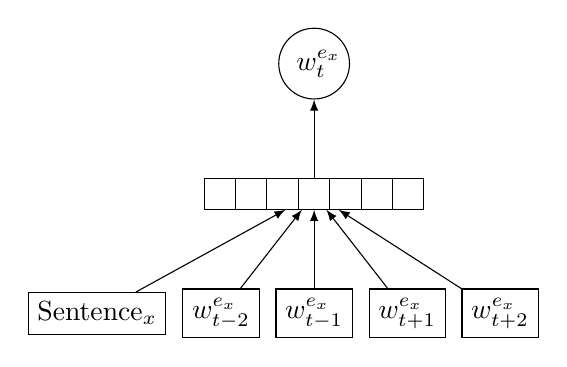
\begin{tikzpicture}[>=latex]
\node[embedding](Sx) {Sentence$_x$};
\node[embedding](We1) [right =0.2cm of Sx] {$w^{e_x}_{t-2}$};
\node[embedding](We2) [right =0.2cm of We1] {$w^{e_x}_{t-1}$};
\node[embedding](We4) [right =0.2cm of We2] {$w^{e_x}_{t+1}$};
\node[embedding](We5) [right =0.2cm of We4] {$w^{e_x}_{t+2}$};
\node[hidden] (h1) [above =of We2] {} edge[<-] (Sx)edge[<-] (We1)edge[<-] (We2)edge[<-] (We4)edge[<-] (We5);
\node[index] (We3) [above =of h1] {$w^{e_x}_{t}$} edge [<-] (h1);
\end{tikzpicture}
\caption{Bilingual distributed memory. The same architecture is trained with English context and word prediction replaced by the other language(s).}
\label{f:bilingual_dm}
\end{figure}
\end{dia}



\section{Multilingual Dbow}

\begin{dia}
\begin{figure}

\center
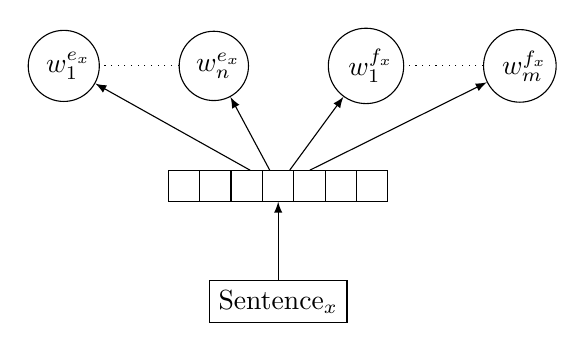
\begin{tikzpicture}[>=latex] 
\node[embedding] (Sx) {Sentence$_x$};
\node[hidden] (h1)[above=of Sx]{} edge [<-] (Sx);
\node[index] (We1) [above left =of h1] {$w^{e_x}_1$} edge [<-] (h1);
\node[index] (Wen) [right =of We1] {$w^{e_x}_n$}edge [<-] (h1) edge [ dotted ] (We1);
\node[index] (Wf1) [right =of Wen] {$w^{f_x}_1$}edge [<-] (h1) ;
\node[index] (Wfm) [right =of Wf1] {$w^{f_x}_m$}edge [<-] (h1) edge [ dotted ] (Wf1);
\end{tikzpicture}
\caption{Bilingual dbow}
\label{f:bilingual_dbow}
\end{figure}
\end{dia}

\begin{dia}
\begin{itemize}
\item Training a single embedding for parallel sentences
\item Word embeddings are not trained
\item Can be extended to more than two languages
\item Results in `good' sentence embeddings (without a compositional model)
\end{itemize}
\end{dia}

\begin{dia}
\begin{itemize}
\item Use the sentence embeddings to obtain word vector: 
\begin{equation*}
emb(w)=\frac{1}{freq(w,D)}\sum_{s\in D}freq(w,s) emb(s)
\end{equation*}
\item Quite good performance (as we will see later)
\end{itemize}
\end{dia}

\begin{dia}
\begin{itemize}
\item Recall the model by Hermann and Blunsom: 
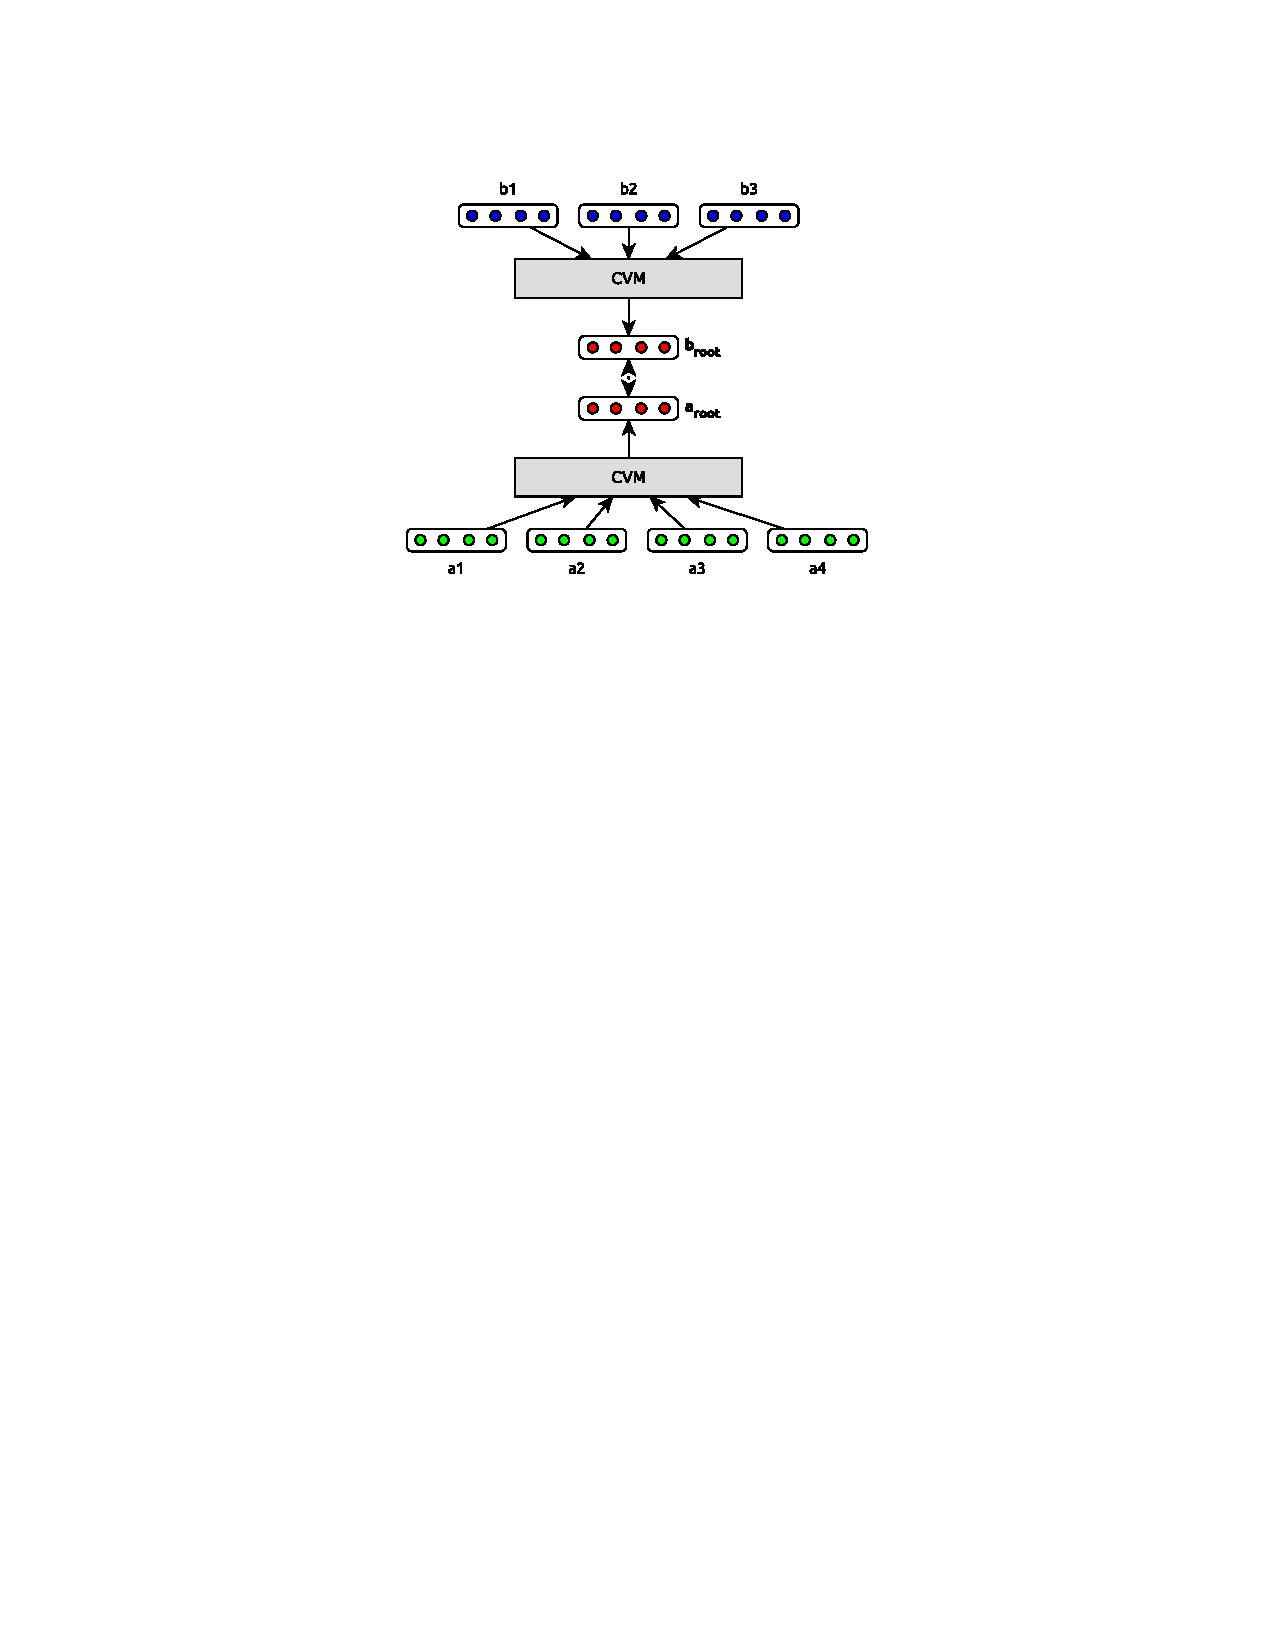
\includegraphics[width=.7\linewidth]{figures/hermannBlunsom}
\end{itemize}
\end{dia}

\begin{dia}
\begin{itemize}
\item We could have a similar training procedure
\item Only: we are not training the sentences, but assume fixed `gold standard' sentence embeddings
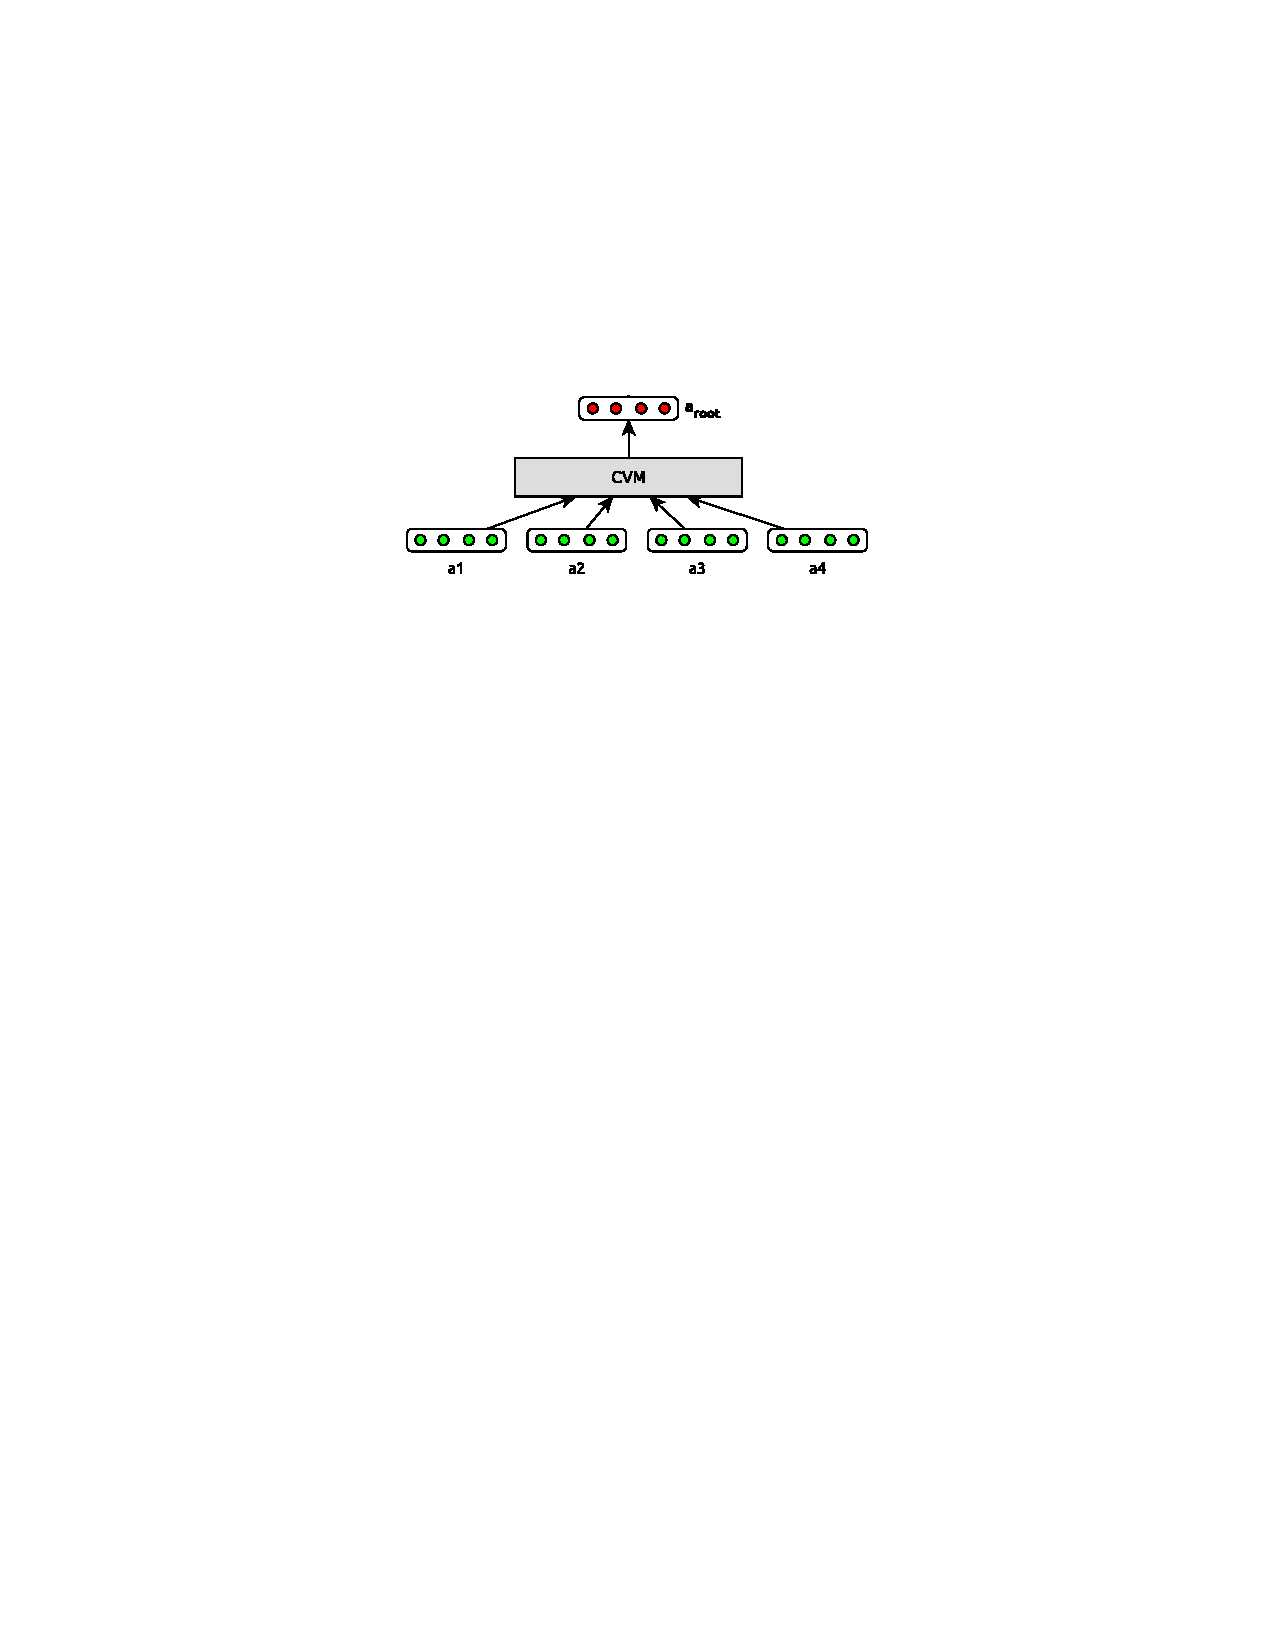
\includegraphics[width=.7\linewidth]{figures/hermannBlunsomHalf}
\item So, we could plug in any compositional model 
\end{itemize}
\end{dia}




\section{Evaluation}
\begin{dia}
\begin{itemize}
\item Training word embeddings: on Europarl data (50k or 500k sentences)
\item Monolingual (English) evaluation: analogy task
\item Crosslingual evaluation: document classification
\end{itemize}
\end{dia}




\begin{dia}
Crosslingual Doccument classification:
\begin{itemize}
\item Given word embeddings, obtain document representation for train and test documents in all languages
\begin{equation*}
emb(doc)=\sum_{w\in doc} idf(w)*emb(w)
\end{equation*}
\item Train a classifier (averaged perceptron) on the training document representations for one language
\item Test classifier performance on the test document representations for another language
\end{itemize}
\end{dia}


%\begin{dia}
%\begin{tabular}{p{.2\textwidth}|p{.35\textwidth} p{.35\textwidth}}
%&RCV & TED\\\hline\hline
%Language &English-German & Many  \\\hline
%Classification& Multiclass:& Binary:\\
% &one topic per document & postive and negative examples for topic \\\hline
%Performance &Accuracy & F1\\\hline
%Baseline &Majority class & ??
%\end{tabular}
%\end{dia}

\begin{dia}
RCV (Reuters) data:
\begin{itemize}
\item English-German
\item Multiclass classification: \\
each document is assigned a single class (topic)
\item Performance measure: accuracy
\item Baseline: majority class
\end{itemize}
\end{dia}


\begin{dia}
TED data:
\begin{itemize}
\item Many languages
\item Binary classification: each class (topic) has positive and negative examples
\item Performance measure: F1 score
\item Baseline: ??
\end{itemize}
\end{dia}

\section{Results}
\begin{dia}
Monolingual evaluation on English:
\begin{table}
\begin{tabular}{l l r r}
 			&vector	&RCV (1000)		&TED		\\
Setting		&length	&accuracy		&F1		\\\hline
Baseline		&		&.468			&.118	 	\\
I-Matrix		&40		&.861			&.154		\\
Paragraph mono	&256		&-			&.399		\\
Paragraph bi 	&256		&-			&.438		\\
Paraword mono	&256		&.866			&.186		\\
Paraword bi 		&256		&.898			&.216		\\
Paraword multi 	&256		&.903			&.245		\\	
Google News		&300		&.951			&.486		\\
\end{tabular}
\end{table}
\end{dia}


\begin{dia}
\begin{itemize}
\item Word vectors as average of the dbow-trained sentences they occur in.
\item Sentences trained on 50k Europarl data in specified languages.
\item Mono- and bilingual evaluation on TED data (F1 scores):
\end{itemize}
\begin{table}
\begin{tabular}{c | r|r r r r }
Sentences 		&sentence	&	\multicolumn{4}{c}{Classification [train]-[test]}	\\
trained on: 		&quality	&EN-EN	&DE-DE	&EN-DE	&DE-EN	\\\hline
EN			&.399		&.186		&.134		&.084		&.153		\\
DE			&.381		&.132		&.091		&.076		&.132	\\
DE-EN			&.622		&.216		&.189		&.201		&.220		\\
multi 			&		&.404		&.368		&.387		&.339		\\
\end{tabular}
\end{table}
\end{dia}

%\begin{dia}
%\begin{itemize}
%\item Word vectors as average of the dbow-trained sentences they occur in.
%\item Sentences trained on 50k Europarl data in specified languages.
%\item Mono- and bilingual evaluation on RCV data with 10000 training examples (accuracy):
%\end{itemize}
%\begin{table}
%\begin{tabular}{c |r r r r }
%Sentences 		&	\multicolumn{4}{c}{Classification train-test}	\\
%trained on: 		&EN-EN	&DE-DE	&EN-DE	&DE-EN	\\\hline
%EN			&.866		&.456		&.398		&.661		\\
%DE			&.850		&.449		&.389		&.704		\\
%DE-EN			&.898		&.467		&.415		&.708		\\
%multi 			&.903		&.473		&.431		&.705		\\
%\end{tabular}
%\end{table}
%\end{dia}






\begin{dia}
\begin{itemize}
\item Word vectors as average of the dbow-trained sentences they occur in.
\item Sentences trained on 50k Europarl data in all languages.
\item multilingual evaluation on TED data (F1 scores):
\end{itemize}
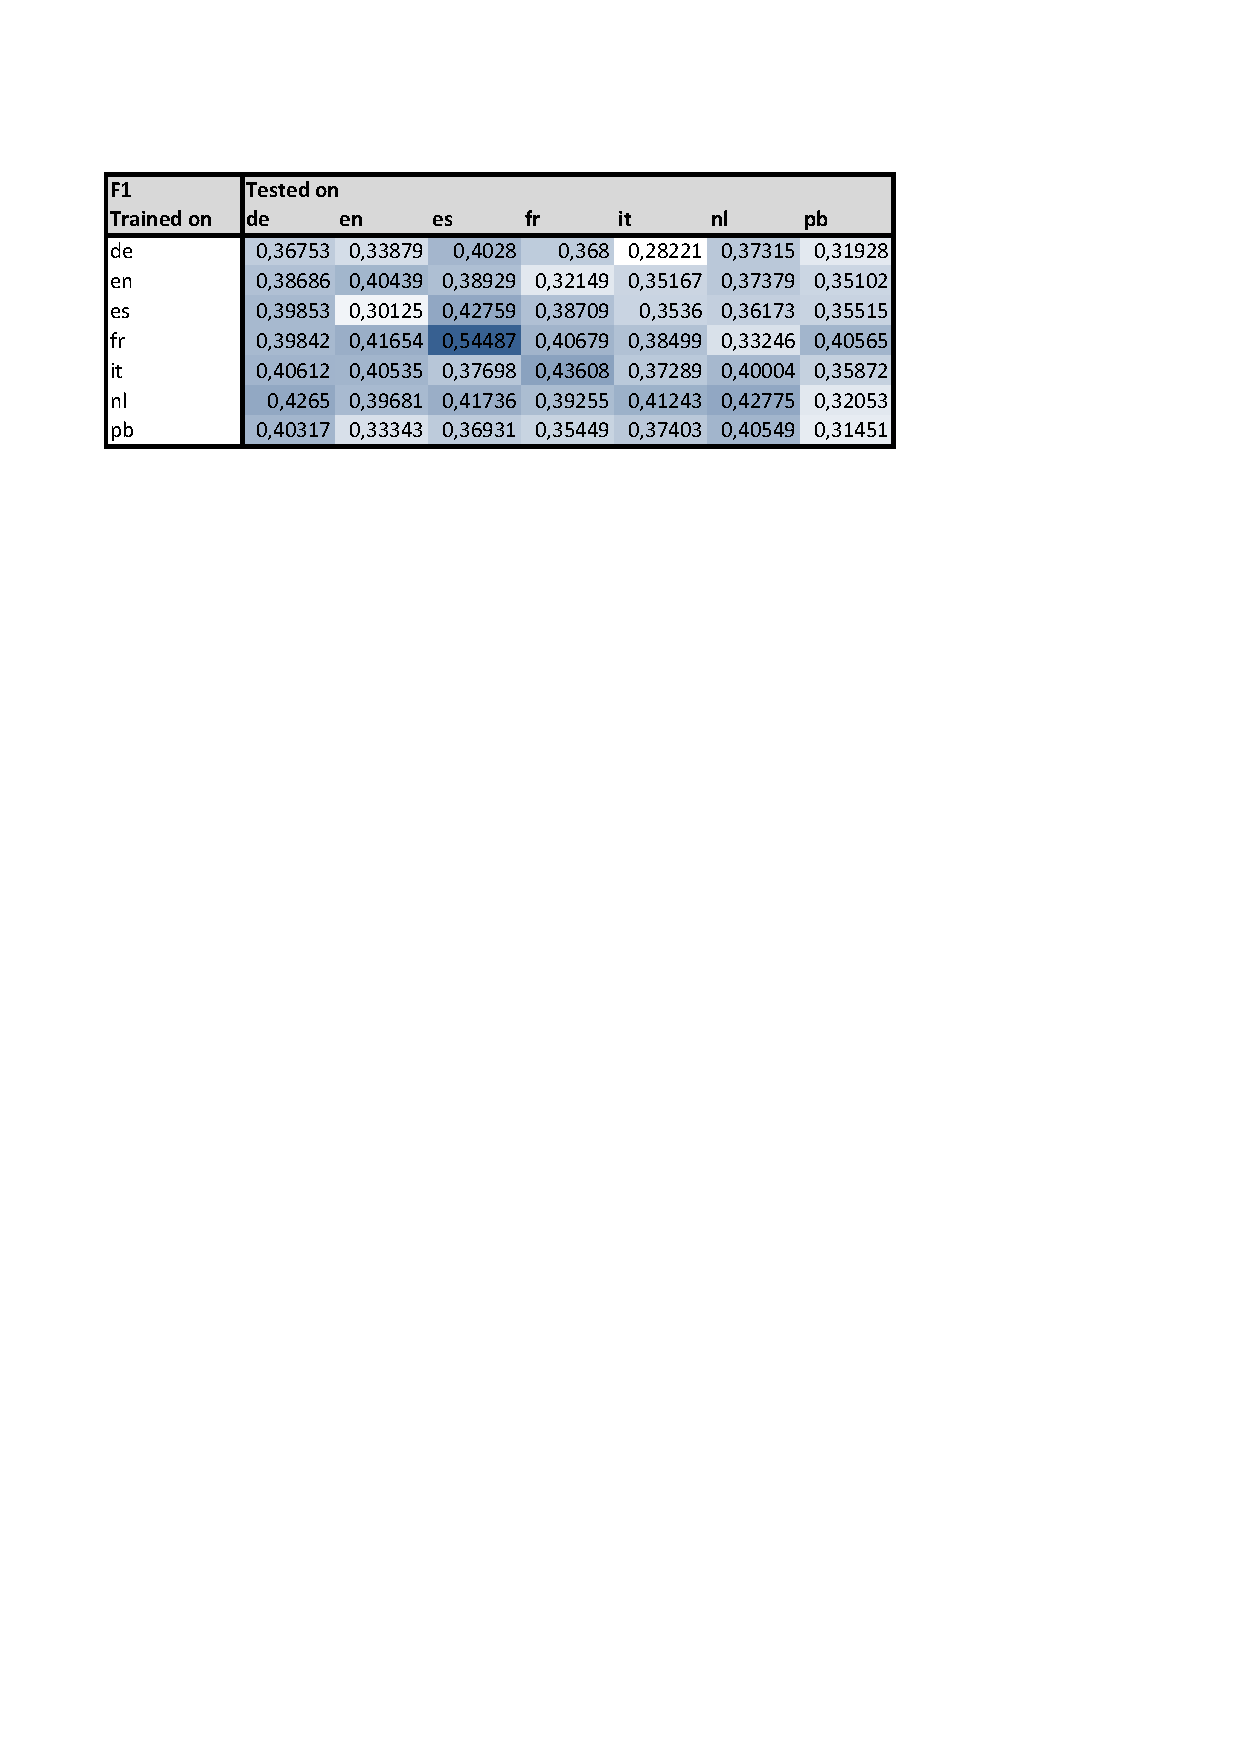
\includegraphics[width=\textwidth]{figures/multilingdbow}
\end{dia}

\section{Graphics and concluding words}
% all parawords multi

\begin{dia}
Words from \emph{multilingual} dbow paragraphs (7 languages)
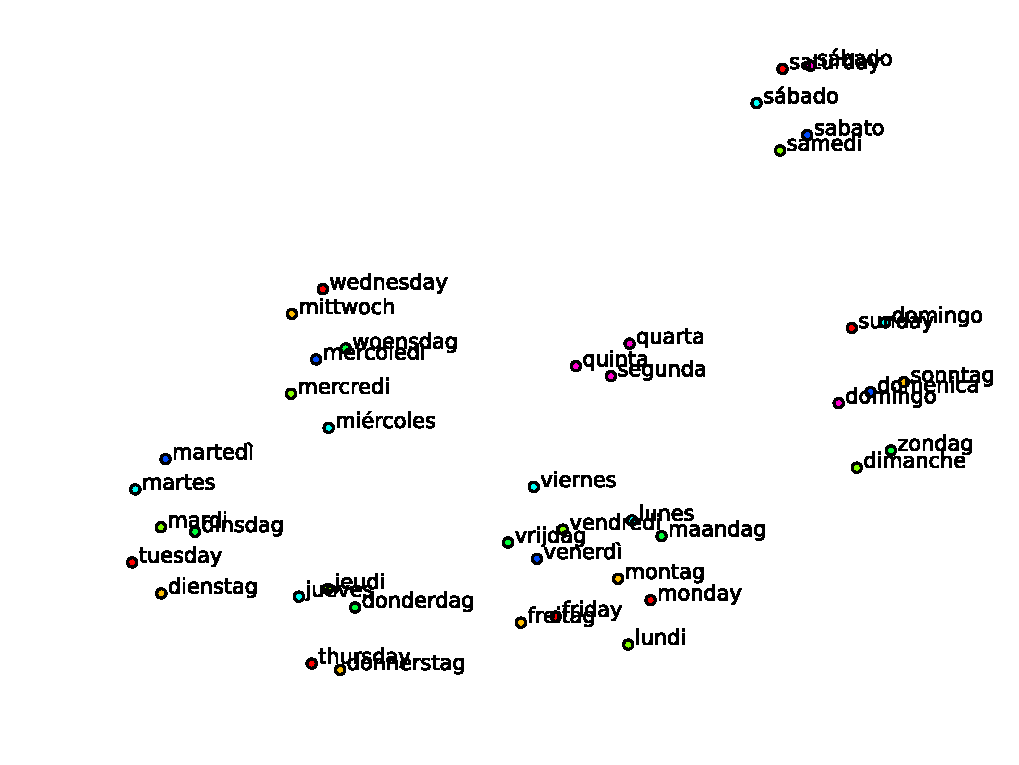
\includegraphics[width=1\linewidth]{figures/weekdays7}
\end{dia}

\begin{dia}
Words from \emph{multilingual} dbow paragraphs (7 languages)
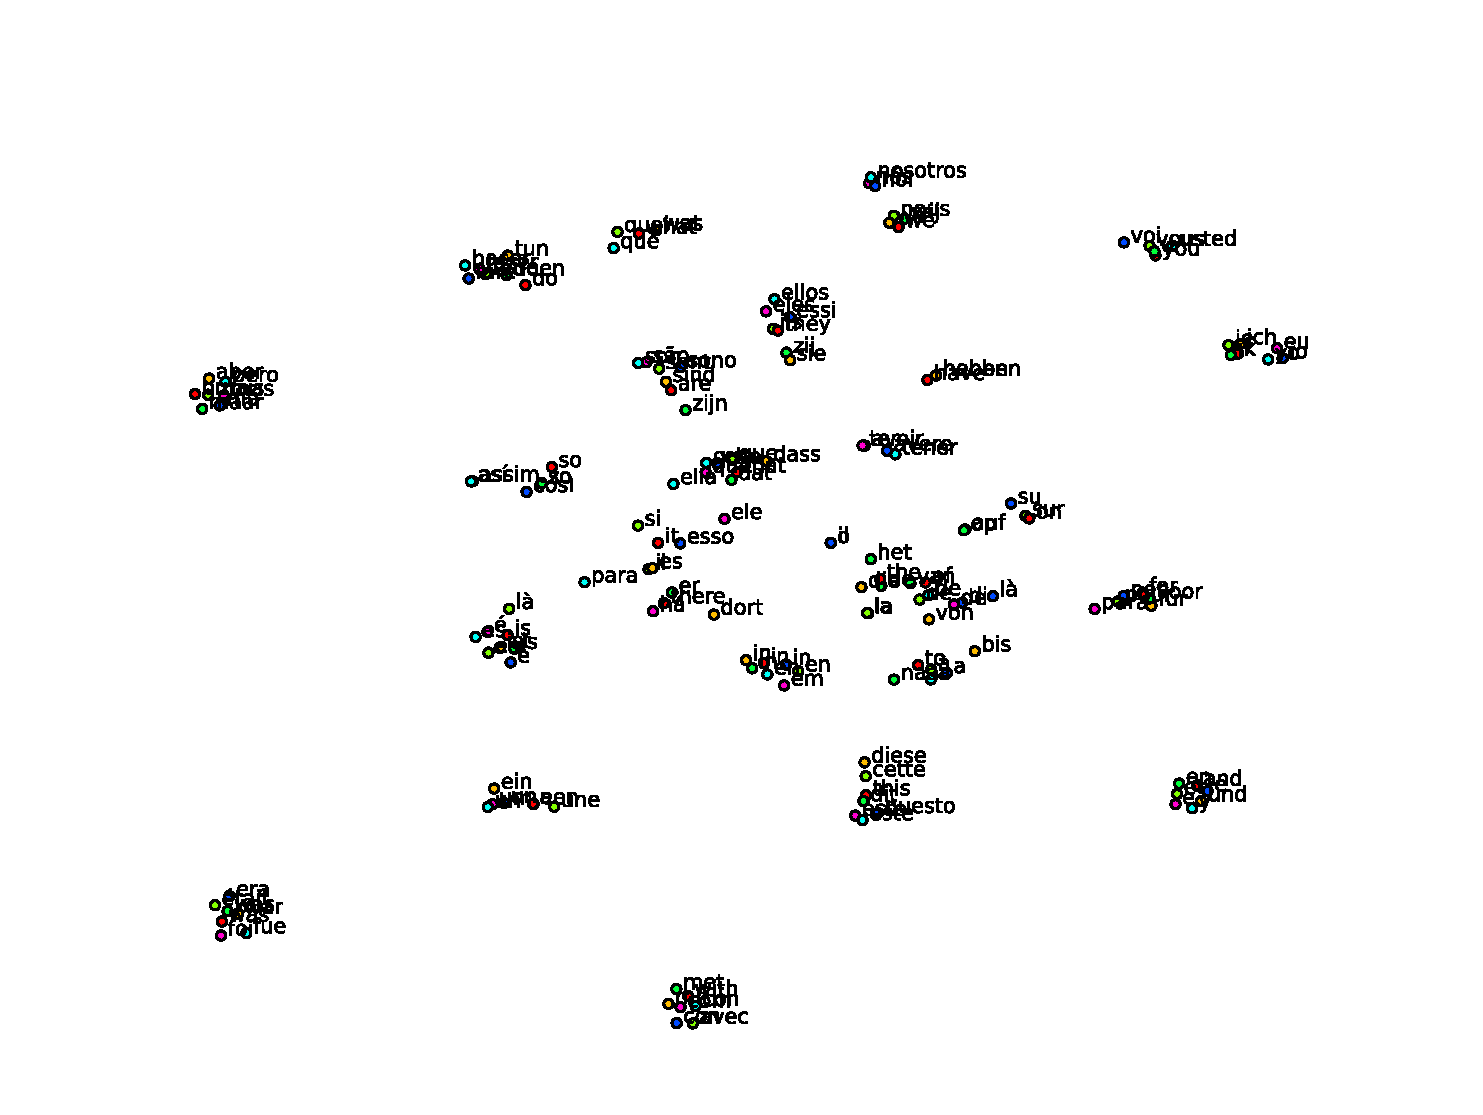
\includegraphics[width=1\linewidth]{figures/en25freq7}
\end{dia}

\begin{dia}
Words from \emph{English transfer} dbow paragraphs (7 languages)
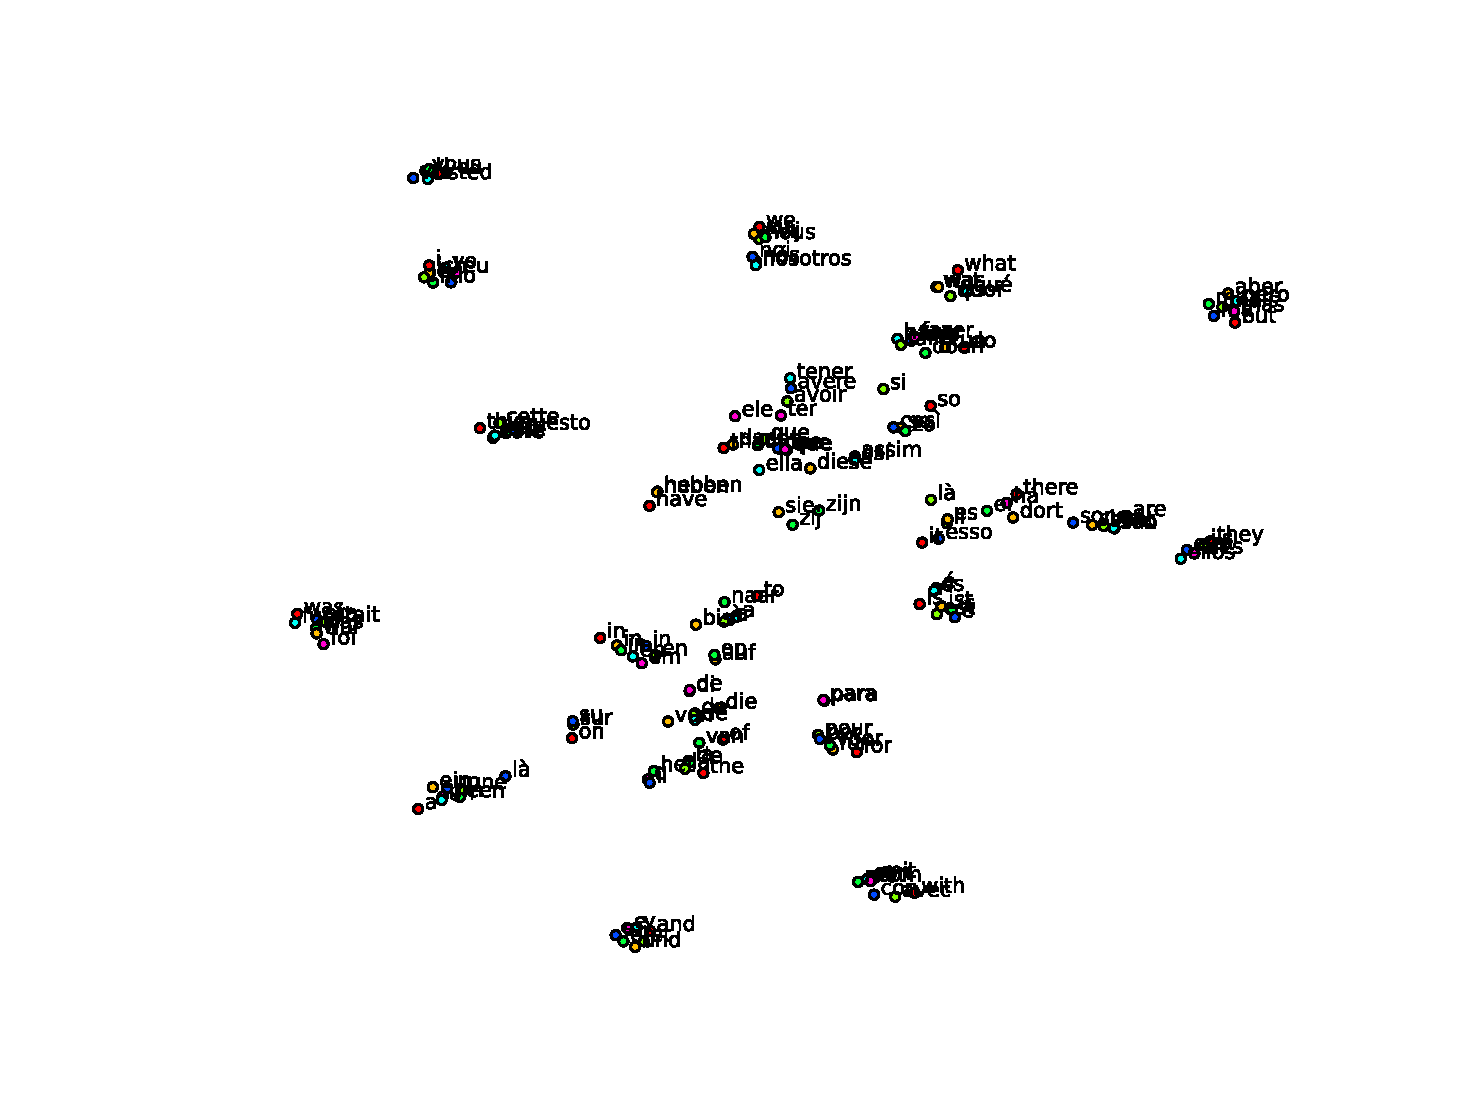
\includegraphics[width=1\linewidth]{figures/transfer_en25freq7}
\end{dia}

\section{Discussion}
\subsection*{F1 baseline}

\begin{dia}
\begin{align*}
Prec=&\frac{TP}{TP+FP}, \\
Rec=&\frac{TP}{TP+FN}, \\
Acc=&\frac{TP+TN}{TP+FP+TN+FN}\\
\text{Majority class:}\\
 neg>pos\rightarrow& \begin{cases}Acc=\frac{TP+TN}{TP+FP+TN+FN}=\frac{TN}{TN+FN}=\frac{neg}{total}\\Prec=\frac{TP}{TP+FP}=0\rightarrow F1=0\end{cases}
\end{align*}
\end{dia}
\begin{dia}
Now assume a stochastic classifier: \\
$P=P(pos)=\frac{pos}{total}$, $P(neg)=1-P$\\

$pos=P*|X|, neg=(1-P)*|X|$
\begin{align*}
TP=&P*pos=P^2*|X|\\
FP=&P*neg=P*(1-P)*|X|\\
FN=&(1-P)*pos=(1-P)*P*|X|\\
F1=&\frac{2*TP}{2*TP+FN+FP}\\
=&\frac{2*P2*|X|}{2*P*P*|X|+(1-P)*P*|X|+(1-P)*P*|X|}\\
=&\frac{2*P^2}{2*P^2+(1-P)*P+(1-P)*P}\\
=&\frac{2*P}{2*P+(1-P)+(1-P)}=\frac{2P}{2}=P\\
\end{align*}
Is $P$ a reasonable F1 baseline?
\end{dia}

\end{document}
